\chapter{Implementation}
This chapter explains the implementation of the system. It contains details about how multiple languages are supported, how the security works and some of the difficulties and limitations encountered.

\section{System Overview}
The system was named CELINE, an abbreviation that comes from the descriptive phrase ``Code EvaLuation In .NEt'' (the uppercase letters forming the abbreviation). Figure \ref{fig:SystemOverview} describes an overview of the system. The system uses a web based GUI for listing problems and submitting solutions to them.

\begin{figure}[h]
	\centering
	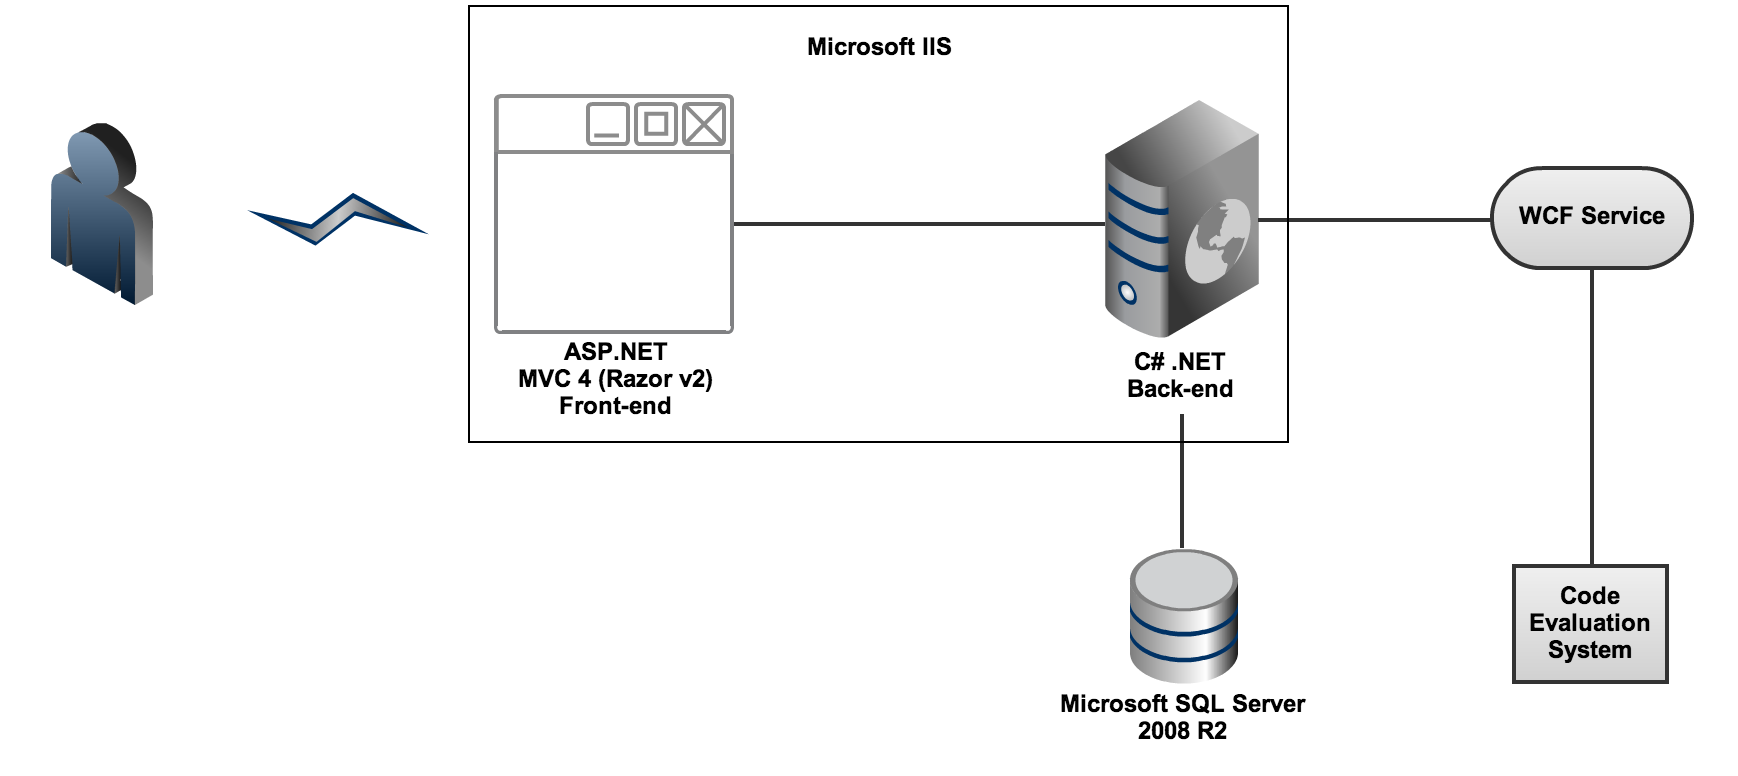
\includegraphics[width=\linewidth]{sections/media/overview.png}
	\caption{Overview of CELINE.}
	\label{fig:SystemOverview}
\end{figure}

Going through this figure from left to right we can see that a user connects to the website, which is built using a combination of ASP.NET MVC4 (Razor v2) technology and JavaScript. The system uses Microsoft IIS to enable this web support, which the standard web server software used in .NET. When the user submits code to solve a problem, that submission is saved to a database which is a Microsoft SQL Server 2008 R2 database. The submission is then forwarded to a WCF Service which in turn creates a new instance of the code evaluation system (built using C\#) using the submission as input. It then returns the status code generated from the submission. 

\subsection{The Web GUI}
The GUI is built using the ASP.NET MVC4 template. This saved both time and effort while still giving the website an easy to understand simplistic style. 

\begin{figure}[h]
	\centering
	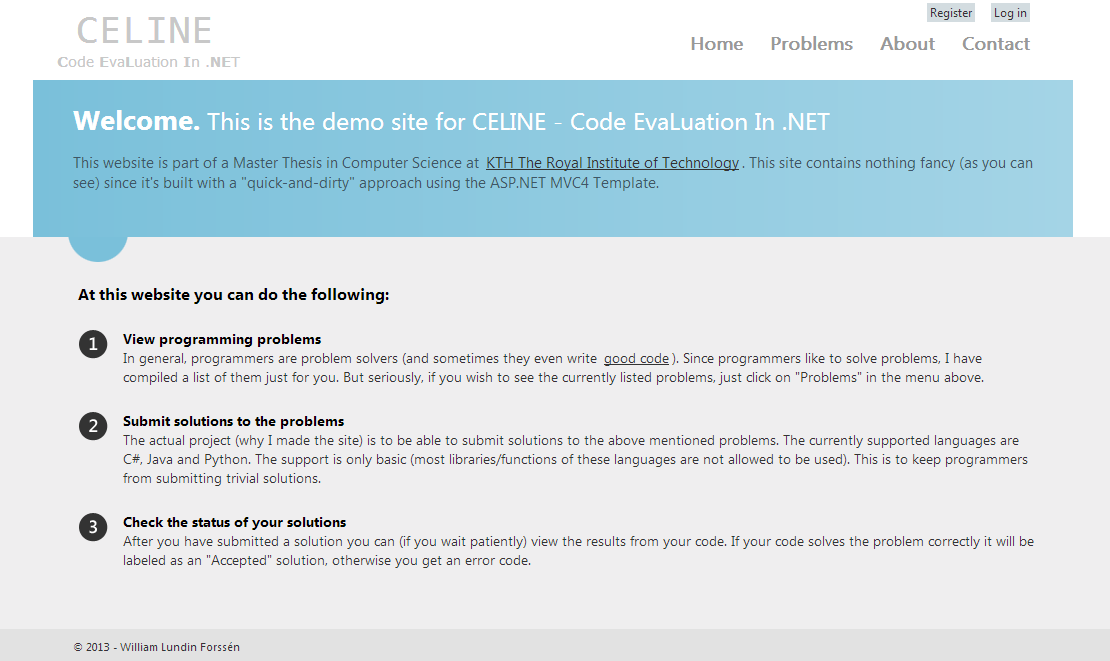
\includegraphics[width=0.75\textwidth]{sections/media/celine_startpage.png}
	\caption{The start page of CELINE.}
	\label{fig:celine_startpage}
\end{figure}

In Figure \ref{fig:celine_startpage} we see the start page. The middle area contains some informative text, the top right contains the site menu, the register and login buttons.

\begin{figure}[h]
\centering
\mbox{
	\subfigure[List of available problems.]{
		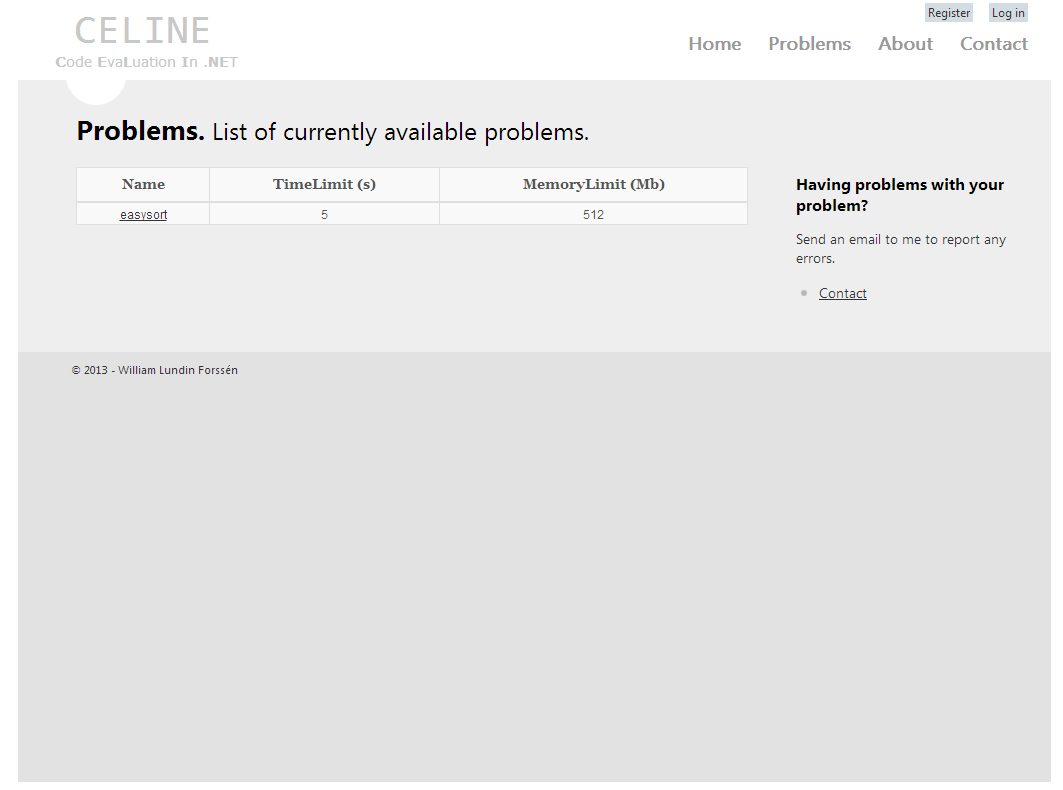
\includegraphics[width=0.48\textwidth]{sections/media/celine_listproblems.png}
	}
	\subfigure[One problem called ``easysort''.]{
		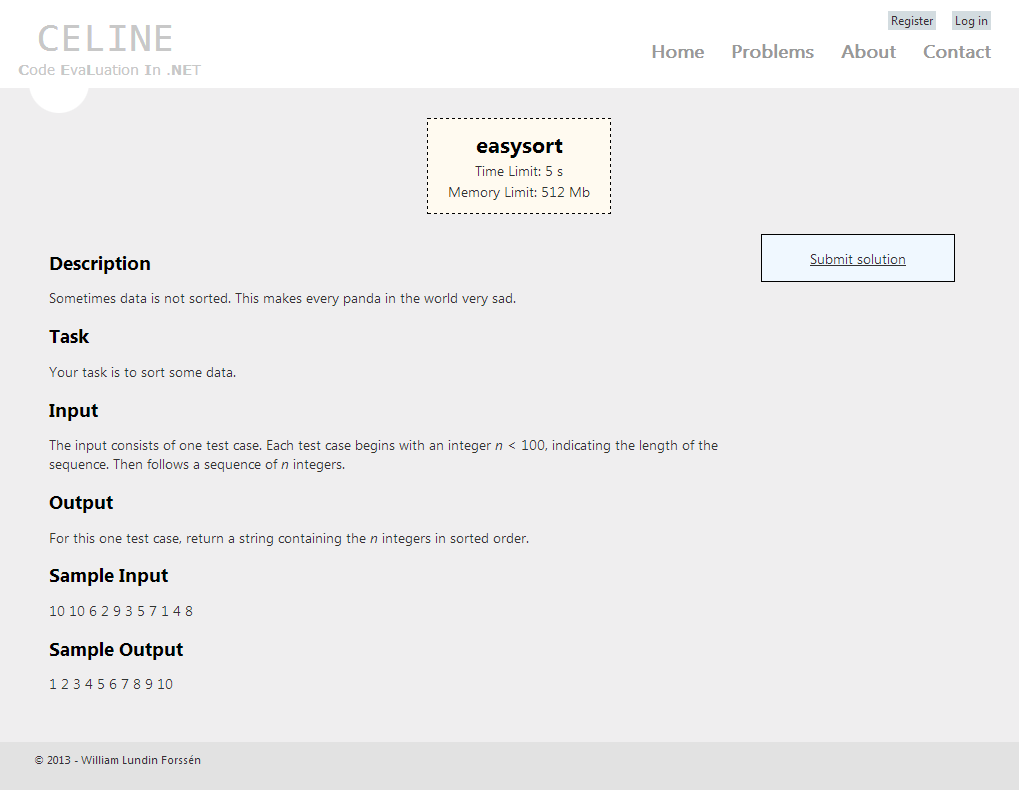
\includegraphics[width=0.48\textwidth]{sections/media/celine_easysort.png} 
	}
}
\caption{Navigating through the problem menu.}
\label{fig:celine_split_problemlist_easysort}
\end{figure}

Figure \ref{fig:celine_split_problemlist_easysort} (a) shows what happens if you click on ``Problems'' in the menu. A list of currently available problems is displayed. The list contains details such as maximum run time and maximum memory usage. 


\subsection{The status codes}
The status code is a simple message indicating if the submission was successful or not. The message can be one of the following:
\begin{itemize}
	\item Accepted - The code has compiled, run and gave the correct answer.
	\item Wrong Answer - The code has compiled and run but gave the wrong answer.
	\item Server Assembly Error - The CES failed to build an assembly from the codefile, thus making the code unable to run.
	\item Submission Error - Occurs if the code tries to reference a library that isn't available. 
	\item Illegal Operation - Occurs if the CES detects a forbidden system call (i.e. accessing files, using the network etc...).
	\item Class or Function Error - Occurs if the class or method name doesn't correspond to, thus resulting in the CES being unable to invoke the method.
	\item Time Limit Exceeded - The code ran longer than the limit for this particular problem.
	\item Rejected - This is a general error, it indicates that the CES has been unable to determine why the submission failed. 
\end{itemize}

The WCF Service is used to avoid the evaluation system crashing due to stack overflow exceptions which are not possible to try-catch in C\# since version 2.0 (referens  till msdn stackoverflowexception) (workarounds exist but they are discouraged).


\section{IKVM}

\section{IronPython}

\section{Difficulties and limitations}
- AppDomains
- IronPython limitation
- ScriptEngine thing
